%%%%%%%%%%%%%%%%%%%%%%%%%%%%%%%%%%%%%%%%%%%%%%%%%%%%%%%%
% 第5章 実験結果と考察
%%%%%%%%%%%%%%%%%%%%%%%%%%%%%%%%%%%%%%%%%%%%%%%%%%%%%%%%
\chapter{実験結果}
\label{chap:results}

本章では，提案手法の有効性を検証するため，ソースドメインとターゲットドメインにおいて異なる観点から評価を行う．
ソースドメインでは，マルチモーダル表現学習および距離学習が設計通りに機能しているかを確認するため，特徴空間における幾何学的な構造（クラス内・クラス間距離）を重点的に分析する．
一方，ターゲットドメインでは，未知の環境および行動に対する実用性を検証するため，最終的な行動識別精度（ARI，NMI）およびt-SNEによる可視化結果を用いて評価する．

本章では，提案手法の有効性を検証するために実施した3つの実験の結果を報告する．

\section{実験1: ターゲットドメインでの行動分類}
本節では，学習時に一度も提示されていないホッキョクグマ監視映像
に対する提案手法の汎化性能を評価する．
これは，提案手法が未知の環境・行動クラスに対しても有効に機能するかを検証する最も重要な実験である．

\subsection{定量評価結果}
札幌市円山動物園のホッキョクグマデータセットに対するクラスタリング性能を
表\ref{tab:clustering_results_polar}に示す．
比較対象として，以下の4つの条件を設定した：

\begin{itemize}
  \item \textbf{RGB Only}：VideoMAE による外観特徴のみを使用
  \item \textbf{Flow Only}：X3D によるオプティカルフロー特徴のみを使用
  \item \textbf{Gated Fusion (w/o Adv)}：提案する Gated Fusion を適用するが，敵対的学習は行わない
  \item \textbf{Proposed (Full)}：Gated Fusion と敵対的学習の両方を適用（提案手法）
\end{itemize}

\begin{table}[t]
  \centering
  \caption{ホッキョクグマ監視映像に対する各手法のクラスタリング性能比較}
  \label{tab:clustering_results_polar}
  \begin{tabular}{lcc}
    \hline
    手法 & ARI & NMI \\
    \hline \hline
    RGB Only & 0.093 & 0.278 \\
    Flow Only & 0.557 & 0.539 \\
    Gated Fusion (w/o Adv) & 0.615 & 0.622 \\
    \textbf{Proposed (Full)} & \textbf{0.742} & \textbf{0.728} \\
    \hline
  \end{tabular}
\end{table}

表\ref{tab:clustering_results_polar}より，以下の知見が得られた：

\paragraph{外観特徴のドメイン依存性}
RGB 特徴のみを用いた場合，ARI は 0.093 と極めて低い結果となった．
この著しい性能低下は，学習データ（ドキュメンタリー映像）と評価データ（監視カメラ映像）の間で生じる
背景環境や照明条件といったドメインシフトの影響によるものと推察される．
VideoMAE は優れた時空間表現能力を有するが，ドメイン間の乖離が大きい場合，
行動固有の特徴よりも背景情報に過剰適合する傾向が見られ，単独での汎化には限界があることが示唆された．

\paragraph{運動特徴のドメイン不変性}
一方，オプティカルフロー特徴のみを用いた場合，ARI は 0.557 まで大幅に改善した．
オプティカルフローは動物のテクスチャや背景情報の影響を受けにくく，
純粋な動作情報を抽出できるため，ドメイン変化に対して高い頑健性を示したと考えられる．
この結果は，未知環境への汎化において，運動情報がドメイン不変な重要な手がかりとなることを裏付けている．

\paragraph{適応的特徴統合の有効性}
Gated Fusion を用いて両モダリティを統合したモデルは，ARI 0.615 を達成した．
これは，運動特徴の頑健性を維持しつつ，外観特徴に含まれる文脈情報を適応的に補完することで，
単一モダリティでは識別困難な複雑な行動パターンに対しても表現力が向上したためと解釈できる．

\paragraph{敵対的学習による種不変表現の獲得}
最終的な提案手法（Full）は ARI 0.742，NMI 0.728 と，比較手法の中で最も高い性能を記録した．
単純な特徴統合（Gated Fusion）と比較して ARI が 0.127 ポイント向上した点は，
敵対的学習が種に特有の情報を効果的に抑制し，
純粋な行動表現の獲得に成功していることを強く示唆している．

\subsection{定性評価結果}

\subsubsection{t-SNE による特徴空間の可視化}
学習された特徴空間の構造を視覚的に分析するため，
各手法による埋め込みを t-SNE により2次元に射影した結果を図\ref{fig:tsne_polar}に示す．
なお，t-SNE は高次元の特徴空間を低次元に射影して可視化する定性的な手法であり，射影時のパラメータ設定によって見え方が変化する性質を持つ．
したがって，本研究では t-SNE の結果はあくまで特徴空間の構造を直感的に理解するための補助的なものと位置づけ，モデルの定量的な性能評価は ARI および NMI に基づいて行う．

\begin{figure}[t]
  \centering
  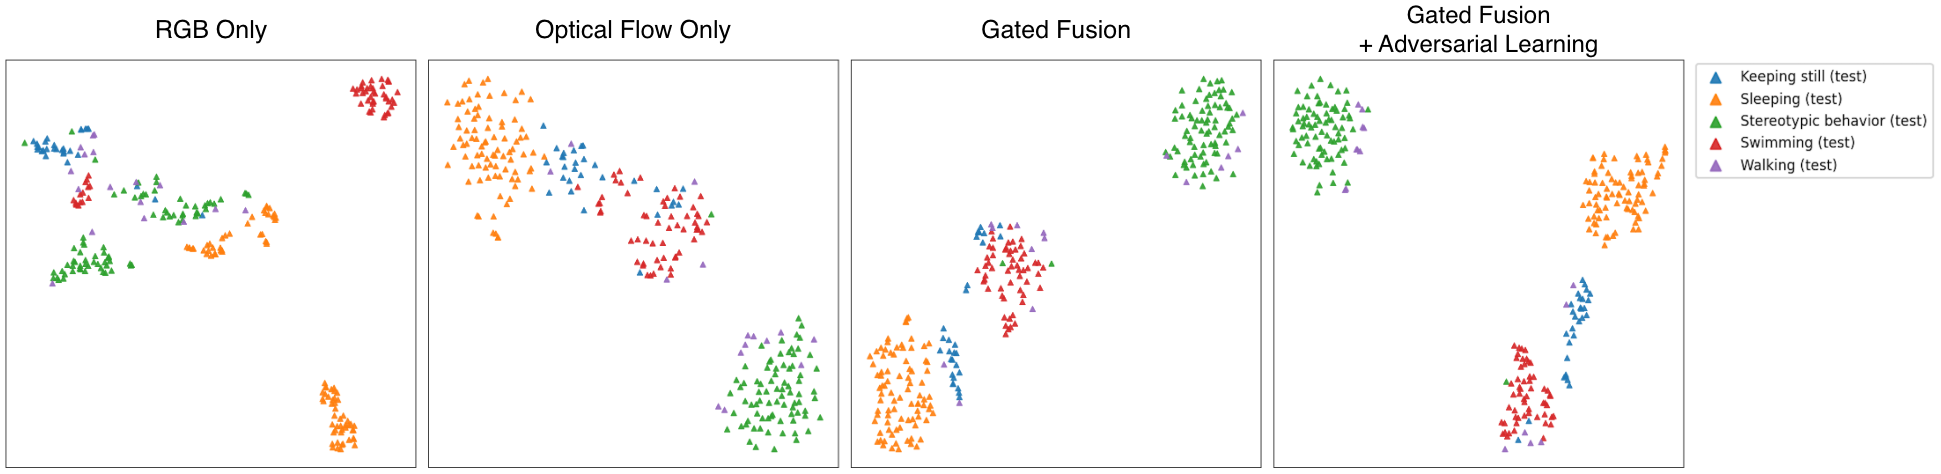
\includegraphics[width=0.9\linewidth]{image/tsne.png}
  \caption{ホッキョクグマデータセットにおける各手法の t-SNE 可視化結果．
    (a) RGB Only，(b) Flow Only，(c) Gated Fusion (w/o Adv)，(d) Proposed (Full)．
    提案手法では各行動クラスが明確に分離されたクラスタを形成している．}
  \label{fig:tsne_polar}
\end{figure}

RGB Only では各行動クラスのサンプルが混在しており，
明確なクラスタ構造が形成されていない．
一方，提案手法（Full）では「Swimming」「Walking」「Sleeping」などの各行動クラスが明確に分離されたクラスタを形成しており，
クラス間の境界も明瞭である．

特に注目すべき点として，動物福祉の観点で重要な
「Stereotypic behavior（常同行動）」のクラスタが，
「Walking」と若干混ざりながらも区別されている．
これは，常同行動が歩行の一種でありながらも，
その反復的なパターンが特徴空間上で識別可能であることを示唆しており，
異常行動の自動検知への応用可能性を示している．

\subsubsection{行動クラス間の誤分類分析}
混同行列および誤分類サンプルの詳細な分析から，以下の2つの主要な課題が明らかになった．

\paragraph{歩行（Walking）と常同行動（Stereotypic behavior）の境界}
一部の「Walking」が「Stereotypic behavior」のクラスタに誤って分類される事例が確認された．
詳細な分析の結果，誤分類された「Walking」クリップの多くには，
30秒間の映像内で「折り返し動作」や「往復するような軌跡」が含まれていた．

本モデルはソースドメイン（Animal Kingdom Dataset）のみで学習されており，「常同行動」という概念を明示的には学習していない．
しかし，結果として特徴空間上では，「特定位置での往復歩行」という物理的特徴に基づいたクラスタ（常同行動のグループ）が形成されている．
誤分類された通常の「Walking」は，偶然にも常同行動と酷似した位置および軌跡を持っていたため，特徴空間上の距離計算において，通常の歩行クラスタよりもこの常同行動クラスタに近接してしまったと解釈できる．

\paragraph{低運動強度および環境ノイズによる混同}
「Walking」や「Swimming」，および「Keeping still」の間で相互に混同が見られた．
詳細な映像確認の結果，この要因は以下の2点に集約される．
第一に，断続的な動作の影響である．「Walking」中に数秒間立ち止まる動作が含まれる場合，
オプティカルフローの強度が著しく低下し，モデルがこれを「静止（Keeping still）」や「低運動なSwimming」と誤認する事例が散見された．
第二に，視認性の悪さと環境ノイズの影響である．
本データセットは低解像度かつ低フレームレートであるため，微細な遊泳動作（Swimming）の視認が困難であり，
モデルが動物の動きではなく「水面の揺らぎ」を誤って学習している可能性がある．
その結果，水面が穏やかなSwimmingや，逆に背景に動きがあるKeeping stillといった誤分類が生じたと考えられる．

\textbf{今後の展望：} 以上の誤分類分析から，さらなる精度向上には以下の2つの指針が重要であると結論付けられる．
第一に，常同行動特有の「執拗な繰り返し」を捉えるための長期的文脈の導入である．
30秒程度のクリップでは単発の往復と常同的な反復の区別が困難であるため，数分単位の時間幅での頻度解析を行うことが有効であると考えられる．
第二に，環境ノイズや断続的な静止に頑健な特徴抽出を行うための空間的アテンションの活用である．
水面の揺らぎを抑制し，動物領域のみに焦点を当てることで，低解像度映像や低運動時においても安定した行動認識が期待される．



\section{実験2: アジアゾウ監視映像への汎化検証}
本節では，提案手法の汎化性能をさらに検証するため，
ホッキョクグマとは異なる動物種であるアジアゾウの監視映像に対する評価を行う．
これにより，提案手法が特定の動物種に依存しない汎用的な行動認識能力を持つかを確認する．

\subsection{定量評価結果}
アジアゾウ監視映像に対するクラスタリング性能を
表\ref{tab:clustering_results_elephant}に示す．

\begin{table}[t]
  \centering
  \caption{アジアゾウ監視映像に対する各手法のクラスタリング性能比較}
  \label{tab:clustering_results_elephant}
  \begin{tabular}{lcc}
    \hline
    手法 & ARI & NMI \\
    \hline \hline
    RGB Only & 0.212 & 0.423 \\
    Flow Only & 0.214 & 0.437 \\
    Gated Fusion (w/o Adv) & 0.223 & 0.445 \\
    \textbf{Proposed (Full)} & \textbf{0.249} & \textbf{0.473} \\
    \hline
  \end{tabular}
\end{table}

表\ref{tab:clustering_results_elephant}より，アジアゾウデータセットにおいても
提案手法（Proposed Full）が，ARI および NMI の両指標において
比較手法の中で最も高い性能を達成したことが確認された．
ただし，ホッキョクグマデータセット（ARI: 0.742）と比較すると，
性能が低下している．

\subsection{t-SNE による可視化}
アジアゾウデータセットにおける各手法の特徴空間を t-SNE により可視化した結果を図\ref{fig:tsne_elephant}に示す．

\begin{figure}[t]
  \centering
  
\includegraphics[width=0.9\linewidth]{image/elephant_adv.png}
  \caption{アジアゾウデータセットにおける各手法の t-SNE 可視化結果．
    ホッキョクグマと比較してクラスタの分離が不明瞭である．}
  \label{fig:tsne_elephant}
\end{figure}

図\ref{fig:tsne_elephant}から，各行動クラスの分離性について以下の傾向が読み取れる．

まず，「Sleeping（黄）」は右上方に極めて凝集度の高い独立したクラスタを形成しており，他の行動と明確に分離されている．
同様に，「Swimming（青）」も右下方に比較的まとまったクラスタを形成しているが，その近傍には「Keeping still（赤）」のサンプルの一部が近接しており，前節で述べた「低運動による混同」が特徴空間上の距離としても表れている．

一方で，左側に分布する「Walking（橙）」と「Eating（緑）」に注目すると，これらは単一の密なクラスタを形成せず，広範囲に分散している．
さらに，両クラスの分布領域は大きく重複しており，明確な境界線が存在しない．
また，「Keeping still（赤）」が単一の塊にならず，複数の箇所に分散している点は，背景や文脈によって異なる特徴表現が学習されていることを示唆している．

\subsection{ホッキョクグマとの比較分析}
表\ref{tab:comparison_polar_elephant}に，ホッキョクグマとアジアゾウの
両データセットにおける提案手法の性能比較を示す．

\begin{table}[t]
  \centering
  \caption{ホッキョクグマとアジアゾウにおける提案手法の性能比較}
  \label{tab:comparison_polar_elephant}
  \begin{tabular}{lcc}
    \hline
    データセット & ARI & NMI \\
    \hline \hline
    ホッキョクグマ & 0.742 & 0.728 \\
    アジアゾウ & 0.249 & 0.473 \\
    \hline
  \end{tabular}
\end{table}

\paragraph{性能低下の要因分析}
性能低下の主な要因として，本データセットにおける「行動クラス定義の曖昧さ」および「クラス内分散の大きさ」が挙げられる．

ホッキョクグマと比較して，アジアゾウの行動はクラス内のバリエーションが著しく大きい．
具体的には，「Walking」クラスの中に，「一定速度での歩行」だけでなく，「停止を含む緩慢な歩行」や「鼻を高く上げながらの歩行」など，運動強度の異なる多様なサブパターンが混在している．
その一方で，「Eating」クラスにおいても「歩きながら鼻を上げて餌を口に運ぶ」動作が含まれるなど，異なる行動クラス間で視覚的・運動的な類似性が高い動作が存在する．

加えて，「Keeping still」クラスにおける「背景コンテキストへの依存性」も無視できない要因である．
t-SNE 上で本クラスが単一の塊にならず，Swimming や Eating の近傍など複数の箇所に分散している点は，
同じ「静止」というラベルが付与されていても，その背景（水中か陸上か）や文脈によって，
モデルが全く異なる特徴表現を学習してしまっていることを示唆している．

これらの「動作の多様性」と「背景の多様性」が，特徴空間におけるサンプルの凝集を妨げている．
実際，t-SNE の可視化結果（図\ref{fig:tsne_elephant}）で見られた広範な分布の重複や拡散は，
単純なクラス定義では捉えきれないデータの複雑性がそのまま投影された結果であり，
これが他クラスとの境界領域を増大させ，クラスタリング精度（ARI）の低下を招いたと結論付けられる．

\section{実験3: ソースドメイン内での行動分類}
本節では，学習に使用した Animal Kingdom Dataset のテストセットに対する提案手法の性能を評価する．
これにより，提案手法がソースドメイン内において
基本的な行動認識能力を維持しているかを確認する．

\subsection{定量評価結果}
Animal Kingdom Dataset のテストセットに対するクラスタリング性能を
表\ref{tab:clustering_results_ak}に示す．

\begin{table}[t]
  \centering
  \caption{Animal Kingdom Dataset のテストセットに対する各手法のクラスタリング性能比較}
  \label{tab:clustering_results_ak}
  \begin{tabular}{lcc}
    \hline
    手法 & ARI & NMI \\
    \hline \hline
    RGB Only & 0.160 & 0.239 \\
    Flow Only & 0.205 & 0.266 \\
    Gated Fusion (w/o Adv) & 0.238 & 0.285 \\
    \textbf{Proposed (Full)} & \textbf{0.313} & \textbf{0.345} \\
    \hline
  \end{tabular}
\end{table}

ソースドメイン内での評価においても，提案手法が最も高い性能を示した．
特筆すべき点は，敵対的学習を導入した Proposed (Full) が，Gated Fusion (w/o Adv) と比較して
ARI で約 0.075 ポイントの大幅な向上を達成したことである．
通常，ドメイン不変性を学習することは，ソースドメインに対する特化性能を犠牲にする可能性があるが，
本実験では逆に性能が向上する結果となった．

これは，Animal Kingdom Dataset 自体が多様な動物種を含んでいるため，
敵対的学習により種に依存しない普遍的な行動特徴の抽出が促進され，
その結果として，同一ソースドメイン内においても行動分類の精度が向上したと考えられる．
また，RGB Only と比較して Flow Only の性能が高く，運動情報が行動識別に有効であることも確認された．

\subsection{t-SNE による可視化}
学習された特徴空間の構造を視覚的に分析するため，
t-SNE を用いて特徴ベクトルを2次元空間に射影した結果を図\ref{fig:tsne_ak}に示す．
図\ref{fig:tsne_ak}(a) は学習データとテストデータの両方を，
図\ref{fig:tsne_ak}(b) はテストデータのみを可視化したものである．

\begin{figure}[t]
  \centering
  \begin{minipage}{0.48\linewidth}
    \centering
    
\includegraphics[width=\linewidth]{image/split_all.png}
    \subcaption{Train + Test}
  \end{minipage}
  \hfill
  \begin{minipage}{0.48\linewidth}
    \centering
    
\includegraphics[width=\linewidth]{image/split_test.png}
    \subcaption{Test only}
  \end{minipage}
  \caption{Animal Kingdom Dataset における特徴空間の t-SNE 可視化．(a) は全データ，(b) はテストデータのみを示す．}
  \label{fig:tsne_ak}
\end{figure}

図\ref{fig:tsne_ak}(b) を参照すると，「Running（橙色）」は特徴空間上の右側に独立したクラスタを形成しており，
他の行動クラスと良好に分離されている．これは，Running が持つ大きな運動エネルギーと一貫した方向性が，特徴空間上で支配的な差異として表現されたためである．

一方で，中央部に位置するクラス群には，明確な境界線が存在せず混在が見られる．この要因は，対象クラスの性質によって以下の2点に大別できる．

第一に，「Eating（緑色）」および「Sensing（紫色）」における動作レポートリーの多様性である．
本実験では対象を哺乳類に限定しているが，それでも種による身体構造や生活様式の違いにより，動作（Motion Repertoire）は著しく異なる．
例えば，「Eating」において，霊長類のように前肢（手）を使って食物を口に運ぶ動物と，草食獣のように直接地面の草を食べる動物では，身体の動きが全く異なる．
同様に「Sensing」においても，後肢で立ち上がり視覚的に周囲を警戒する動作や，地面に鼻を近づけて嗅覚を用いる動作など，多種多様なパターンが含まれる．
このように，同一クラスラベルであっても物理的に類似しない動作が混在していることが，特徴空間上での凝集を妨げ，境界を不明瞭にしている主因である．

第二に，「Walking（水色）」や「Keeping still（青色）」における環境ノイズの影響である．
本データセットには移動カメラによる映像が多く含まれており，カメラのパンやチルトによる「背景全体の動き」がオプティカルフローに混入する．
この背景ノイズが，Walking のような緩慢な動作や Keeping still といった静止状態の微細な運動特徴を埋没させてしまうため，
これら低運動クラス間の識別が困難になったと推察される．

また，図\ref{fig:tsne_ak}(a) において，学習データとテストデータの分布が重なり合っている点は，
モデルが特定のサンプルに過学習することなく，ソースドメイン内での汎化性能を適切に維持していることを示している．

\subsection{種識別器の分類精度}
敵対的学習によって種に依存しない表現が獲得されているかを検証するため，種識別器による分類精度を評価した．
本評価では，比較する手法の学習条件に応じて，以下の2種類の評価方法を適切に使い分けた．

\begin{itemize}
  \item \textbf{Fresh Probing}（Gated Fusion w/o Adv で使用）: \\
  この設定では学習時に種識別器が存在しないため，重みが固定された特徴抽出器から得られる特徴量を用いて，新規に種識別器を学習させ,その精度を評価した．
  これは，「特徴量そのものに動物種の情報がどの程度残留しているか」を純粋に測定するための指標である．

  \item \textbf{Pretrained Discriminator}（Proposed Full で使用）: \\
  この設定では，敵対的学習のプロセスにおいて特徴抽出器と競合関係にあった「学習済みの種識別器」をそのまま用いて評価した．
  これは，「特徴抽出器が敵対する識別器をどの程度うまく欺くことができたか」を示す指標である．
\end{itemize}

表\ref{tab:species_acc}に結果を示す．

\begin{table}[t]
  \centering
  \caption{種識別器による分類精度の比較}
  \label{tab:species_acc}
  \begin{tabular}{lccc}
    \hline
    手法 & 評価方法 & 種識別精度 (\%) & MCC \\
    \hline \hline
    Gated Fusion (w/o Adv) & Fresh Probing & 36.2 & 0.321 \\
    \textbf{Proposed (Full)} & \textbf{Pretrained Disc.} & \textbf{10.1} & \textbf{0.036} \\
    \hline
    ランダム推測 & - & 0.6 & 0.000 \\
    \hline
  \end{tabular}
\end{table}

敵対的学習を行わない場合（Gated Fusion w/o Adv），種識別精度は 36.2\%，Matthews 相関係数（MCC）は 0.321 となり，ランダム推測（0.6\%，MCC 0.0）と比較して有意に高い値を示した．
これは，通常の学習では，行動認識において動物種の情報（体型や模様など）が強力な手がかりとして利用されており，特徴ベクトルに種情報が色濃く反映されていることを意味する．

一方，敵対的学習を導入した提案手法（Proposed Full）では，精度が 10.1\%，MCC が 0.036 まで大幅に低下した．MCC が 0 に極めて近いことは，識別器の予測がランダムな推測とほとんど相関がない状態まで無力化されたことを示している．
この結果は，特徴抽出器が識別器を欺くことに成功し，種情報を捨象した境界不変な特徴空間が形成されたことを強く示唆している．

なお，精度が完全なランダム（0.6\%）まで低下しなかった要因として，特定の行動と動物の身体構造には不可分な相関が存在するため，動きの特徴から間接的に種が推測される可能性が残ることが挙げられる．
しかしながら，ベースラインと比較して識別性は著しく抑制されており，この「種情報の忘却」が，結果としてターゲットドメインへの高い汎化性能に寄与したと結論付けられる．


\subsection{特徴空間におけるクラス間距離の分析}

学習された特徴空間における各行動クラスの分離性を定量的に評価するため，
特徴空間上でのクラス間およびクラス内におけるサンプルのユークリッド距離の平均と分散を算出した．
表\ref{tab:distance_mean}に距離の平均値を，表\ref{tab:distance_var}に距離の分散を示す．
表中の対角成分は同一クラス内のサンプルペア間の距離（クラス内距離），
非対角成分は異なるクラス間のサンプルペア間の距離（クラス間距離）を表す．

\begin{table}[t]
  \centering
  \caption{各行動クラス間の特徴空間上での距離平均（対角成分はクラス内距離）}
  \label{tab:distance_mean}
  \resizebox{\columnwidth}{!}{
  \begin{tabular}{lccccccc}
    \hline
     & Attending & Eating & Jumping & Keeping still & Running & Sensing & Walking \\
    \hline \hline
    Attending & 0.755 & 0.833 & 0.861 & 0.786 & 1.021 & 0.834 & 0.888 \\
    Eating & 0.833 & \textbf{0.672} & 1.020 & 0.849 & \textbf{1.120} & 0.892 & 0.903 \\
    Jumping & 0.861 & 1.020 & \textbf{0.648} & 0.831 & 0.762 & 0.872 & 0.813 \\
    Keeping still & 0.786 & 0.849 & 0.831 & 0.680 & 0.942 & 0.763 & \textit{0.746} \\
    Running & 1.021 & \textbf{1.120} & 0.762 & 0.942 & \textbf{0.640} & 0.981 & 0.804 \\
    Sensing & 0.834 & 0.892 & 0.872 & 0.763 & 0.981 & 0.722 & 0.812 \\
    Walking & 0.888 & 0.903 & 0.813 & \textit{0.746} & 0.804 & 0.812 & \textbf{0.648} \\
    \hline
  \end{tabular}
  }
\end{table}

\begin{table}[t]
  \centering
  \caption{各行動クラス間の特徴空間上での距離分散}
  \label{tab:distance_var}
  \resizebox{\columnwidth}{!}{
  \begin{tabular}{lccccccc}
    \hline
     & Attending & Eating & Jumping & Keeping still & Running & Sensing & Walking \\
    \hline \hline
    Attending & 0.084 & 0.061 & 0.066 & 0.054 & 0.069 & 0.054 & 0.066 \\
    Eating & 0.061 & 0.069 & 0.077 & 0.063 & 0.086 & 0.058 & 0.100 \\
    Jumping & 0.066 & 0.077 & 0.084 & 0.059 & 0.064 & 0.054 & 0.067 \\
    Keeping still & 0.054 & 0.063 & 0.059 & 0.085 & 0.103 & 0.054 & 0.079 \\
    Running & 0.069 & 0.086 & 0.064 & 0.103 & \textbf{0.125} & 0.084 & \textbf{0.150} \\
    Sensing & 0.054 & 0.058 & 0.054 & 0.054 & 0.084 & 0.080 & 0.070 \\
    Walking & 0.066 & 0.100 & 0.067 & 0.079 & \textbf{0.150} & 0.070 & 0.102 \\
    \hline
  \end{tabular}
  }
\end{table}

表\ref{tab:distance_mean}の結果から，クラスの分離性について以下の傾向が読み取れる．
第一に，対角成分（クラス内距離）は，非対角成分（クラス間距離）と比較して全体的に小さな値をとっている．
特に「Running」「Jumping」「Walking」といった特徴的な運動を伴うクラスにおいては，
クラス内距離が 0.640--0.648 程度と低く抑えられており，
これらの行動が特徴空間上で高い凝集性を持ってクラスタリングされていることを示している．

第二に，クラス間の距離関係に注目すると，「Eating」と「Running」の間の平均距離は 1.120 と最も大きい．
これは，静的な要素を含む採食行動と，激しい動きを伴う走行行動が，特徴空間上で明確に分離されていることを意味する．
対照的に，「Keeping still（静止）」と「Walking（歩行）」の間の距離は 0.746 と，
異種クラス間であるにもかかわらず，クラス内距離に近い小さな値となった．
これは，ゆっくりとした歩行や立ち止まりかけた状態など，
両者の境界線上にある曖昧な動作が空間上で近接しており，誤分類が生じやすい構造的な要因となっていることを定量的に裏付けている．

また，表\ref{tab:distance_var}の分散分析からは，クラス分布の形状に関する知見が得られる．
特に「Running」に関連する項で分散が顕著に大きい傾向が見られた（クラス内分散：0.125，Walking とのクラス間分散：0.150）．
クラス内分散の大きさは，「Running」というカテゴリ内に多様な速度や姿勢の変化が含まれ，特徴空間上で広く分布していることを示している．
さらに Walking との間の分散が大きいことは，両クラスの距離が一定ではなく，
サンプルによっては極めて近接していることを示唆しており，
これが Running と Walking の分離を困難にする一因であると考えられる．

\subsection{ゲーティングパラメータの分析}
提案手法の Gated Fusion 機構が，
実際にどのように外観・運動特徴を統合しているかを分析するため，
学習過程におけるゲーティングパラメータ $\boldsymbol{\alpha}$ の変化を調査した．
図\ref{fig:alpha_stats}に，学習エポックごとの $\boldsymbol{\alpha}$ の平均値，最大値，最小値，および標準偏差の推移を示す．
ここで，$\boldsymbol{\alpha}$ は運動特徴（Flow）への重みであり，値が大きいほど運動情報を重視することを意味する．

\begin{figure}[t]
  \centering
  \begin{minipage}{0.48\linewidth}
    \centering
    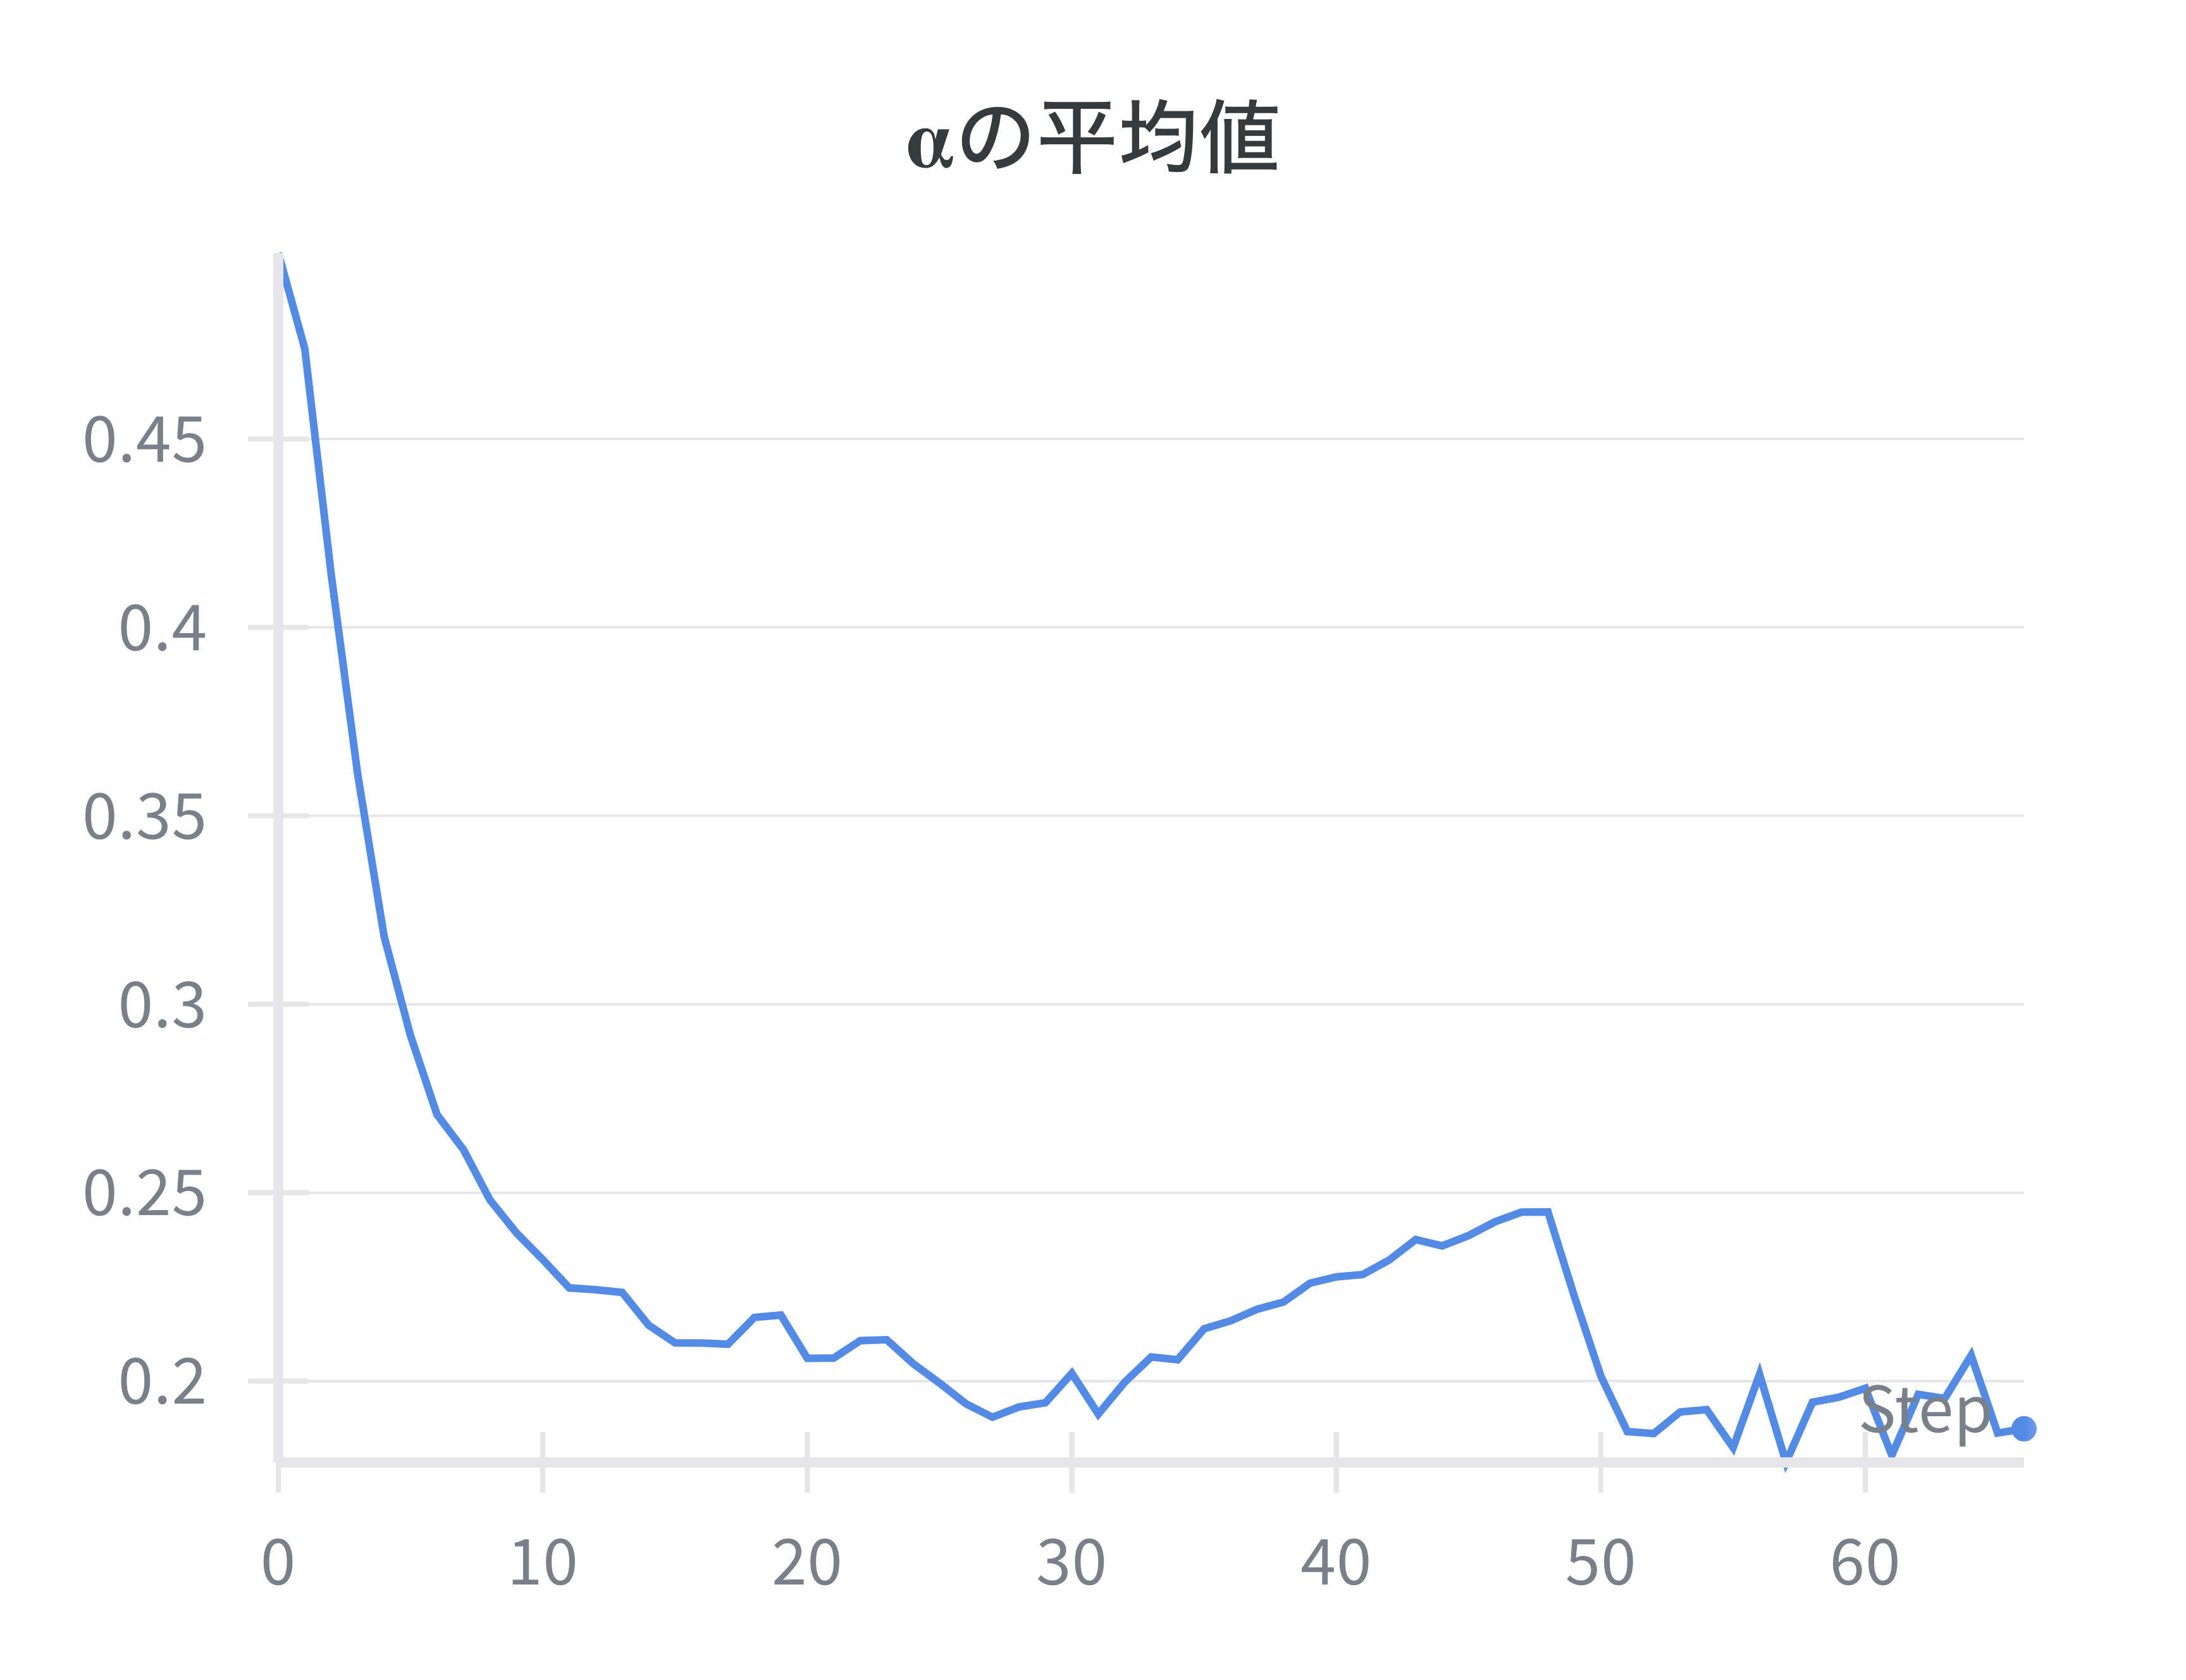
\includegraphics[width=\linewidth]{image/alpha_mean.png}
    \subcaption{Mean of $\boldsymbol{\alpha}$}
  \end{minipage}
  \hfill
  \begin{minipage}{0.48\linewidth}
    \centering
    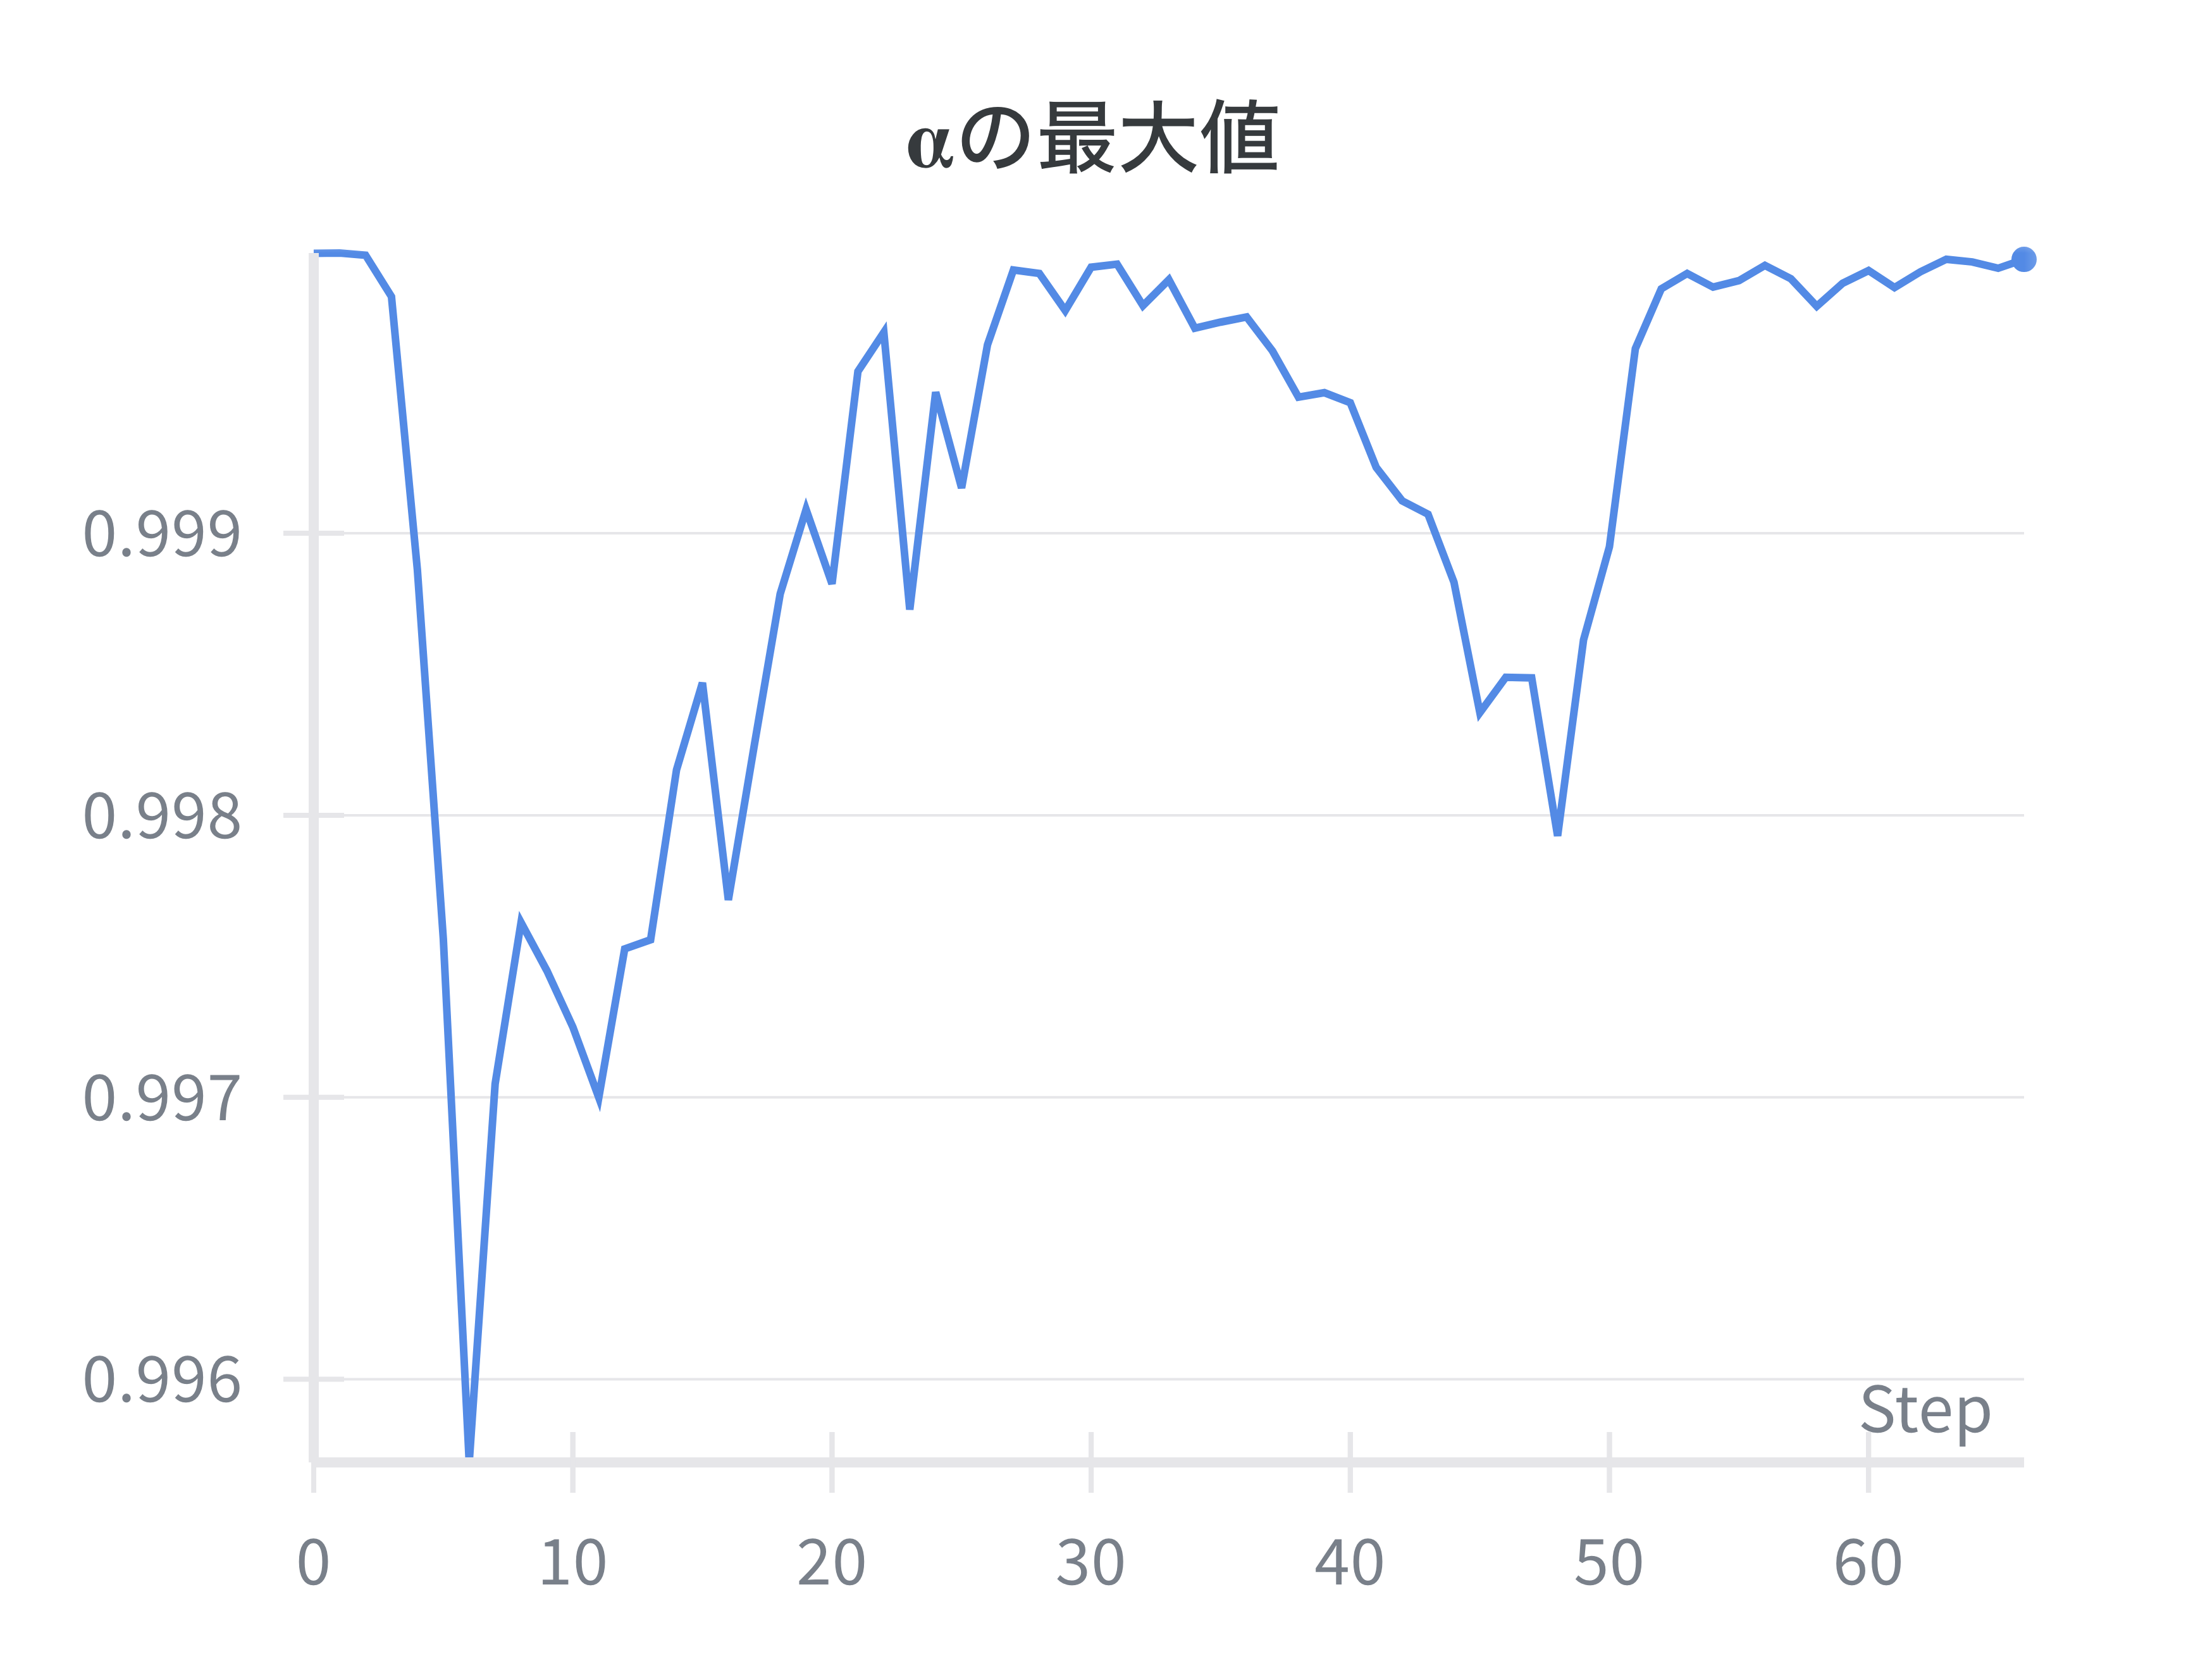
\includegraphics[width=\linewidth]{image/alpha_max.png}
    \subcaption{Max of $\boldsymbol{\alpha}$}
  \end{minipage}
  \vspace{1em} \\ 
  \begin{minipage}{0.48\linewidth}
    \centering
    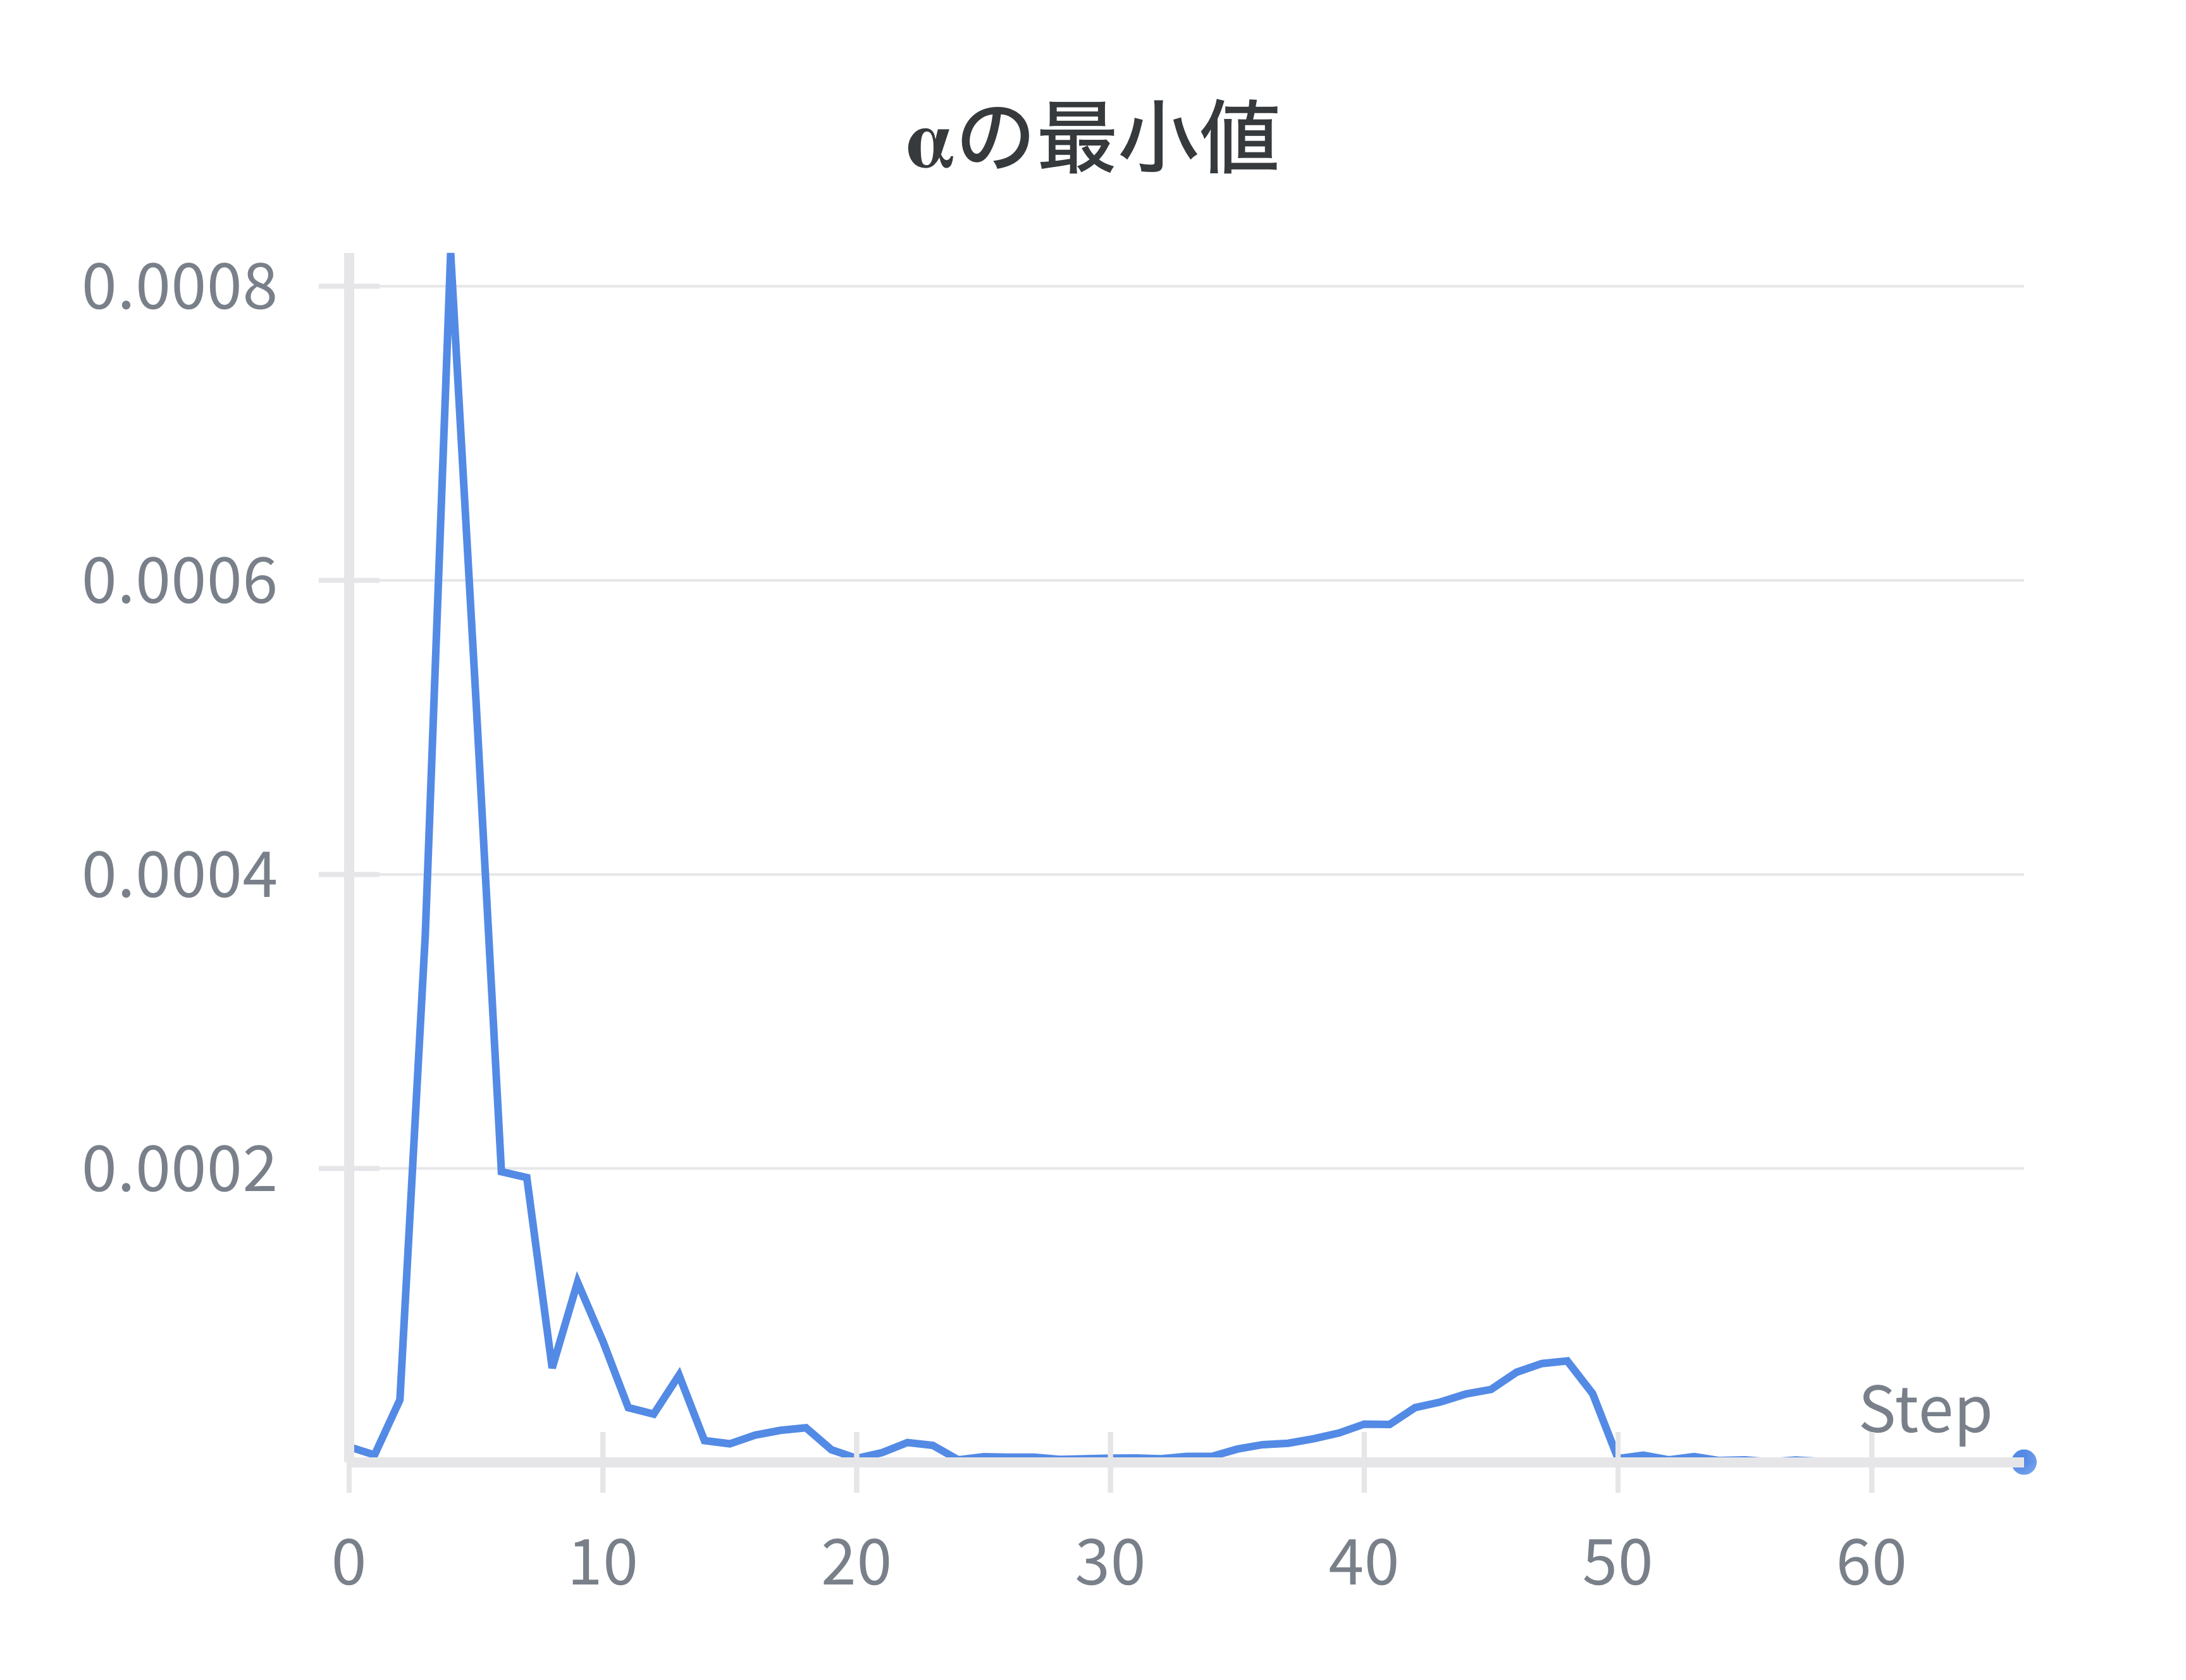
\includegraphics[width=\linewidth]{image/alpha_min.png}
    \subcaption{Min of $\boldsymbol{\alpha}$}
  \end{minipage}
  \hfill
  \begin{minipage}{0.48\linewidth}
    \centering
    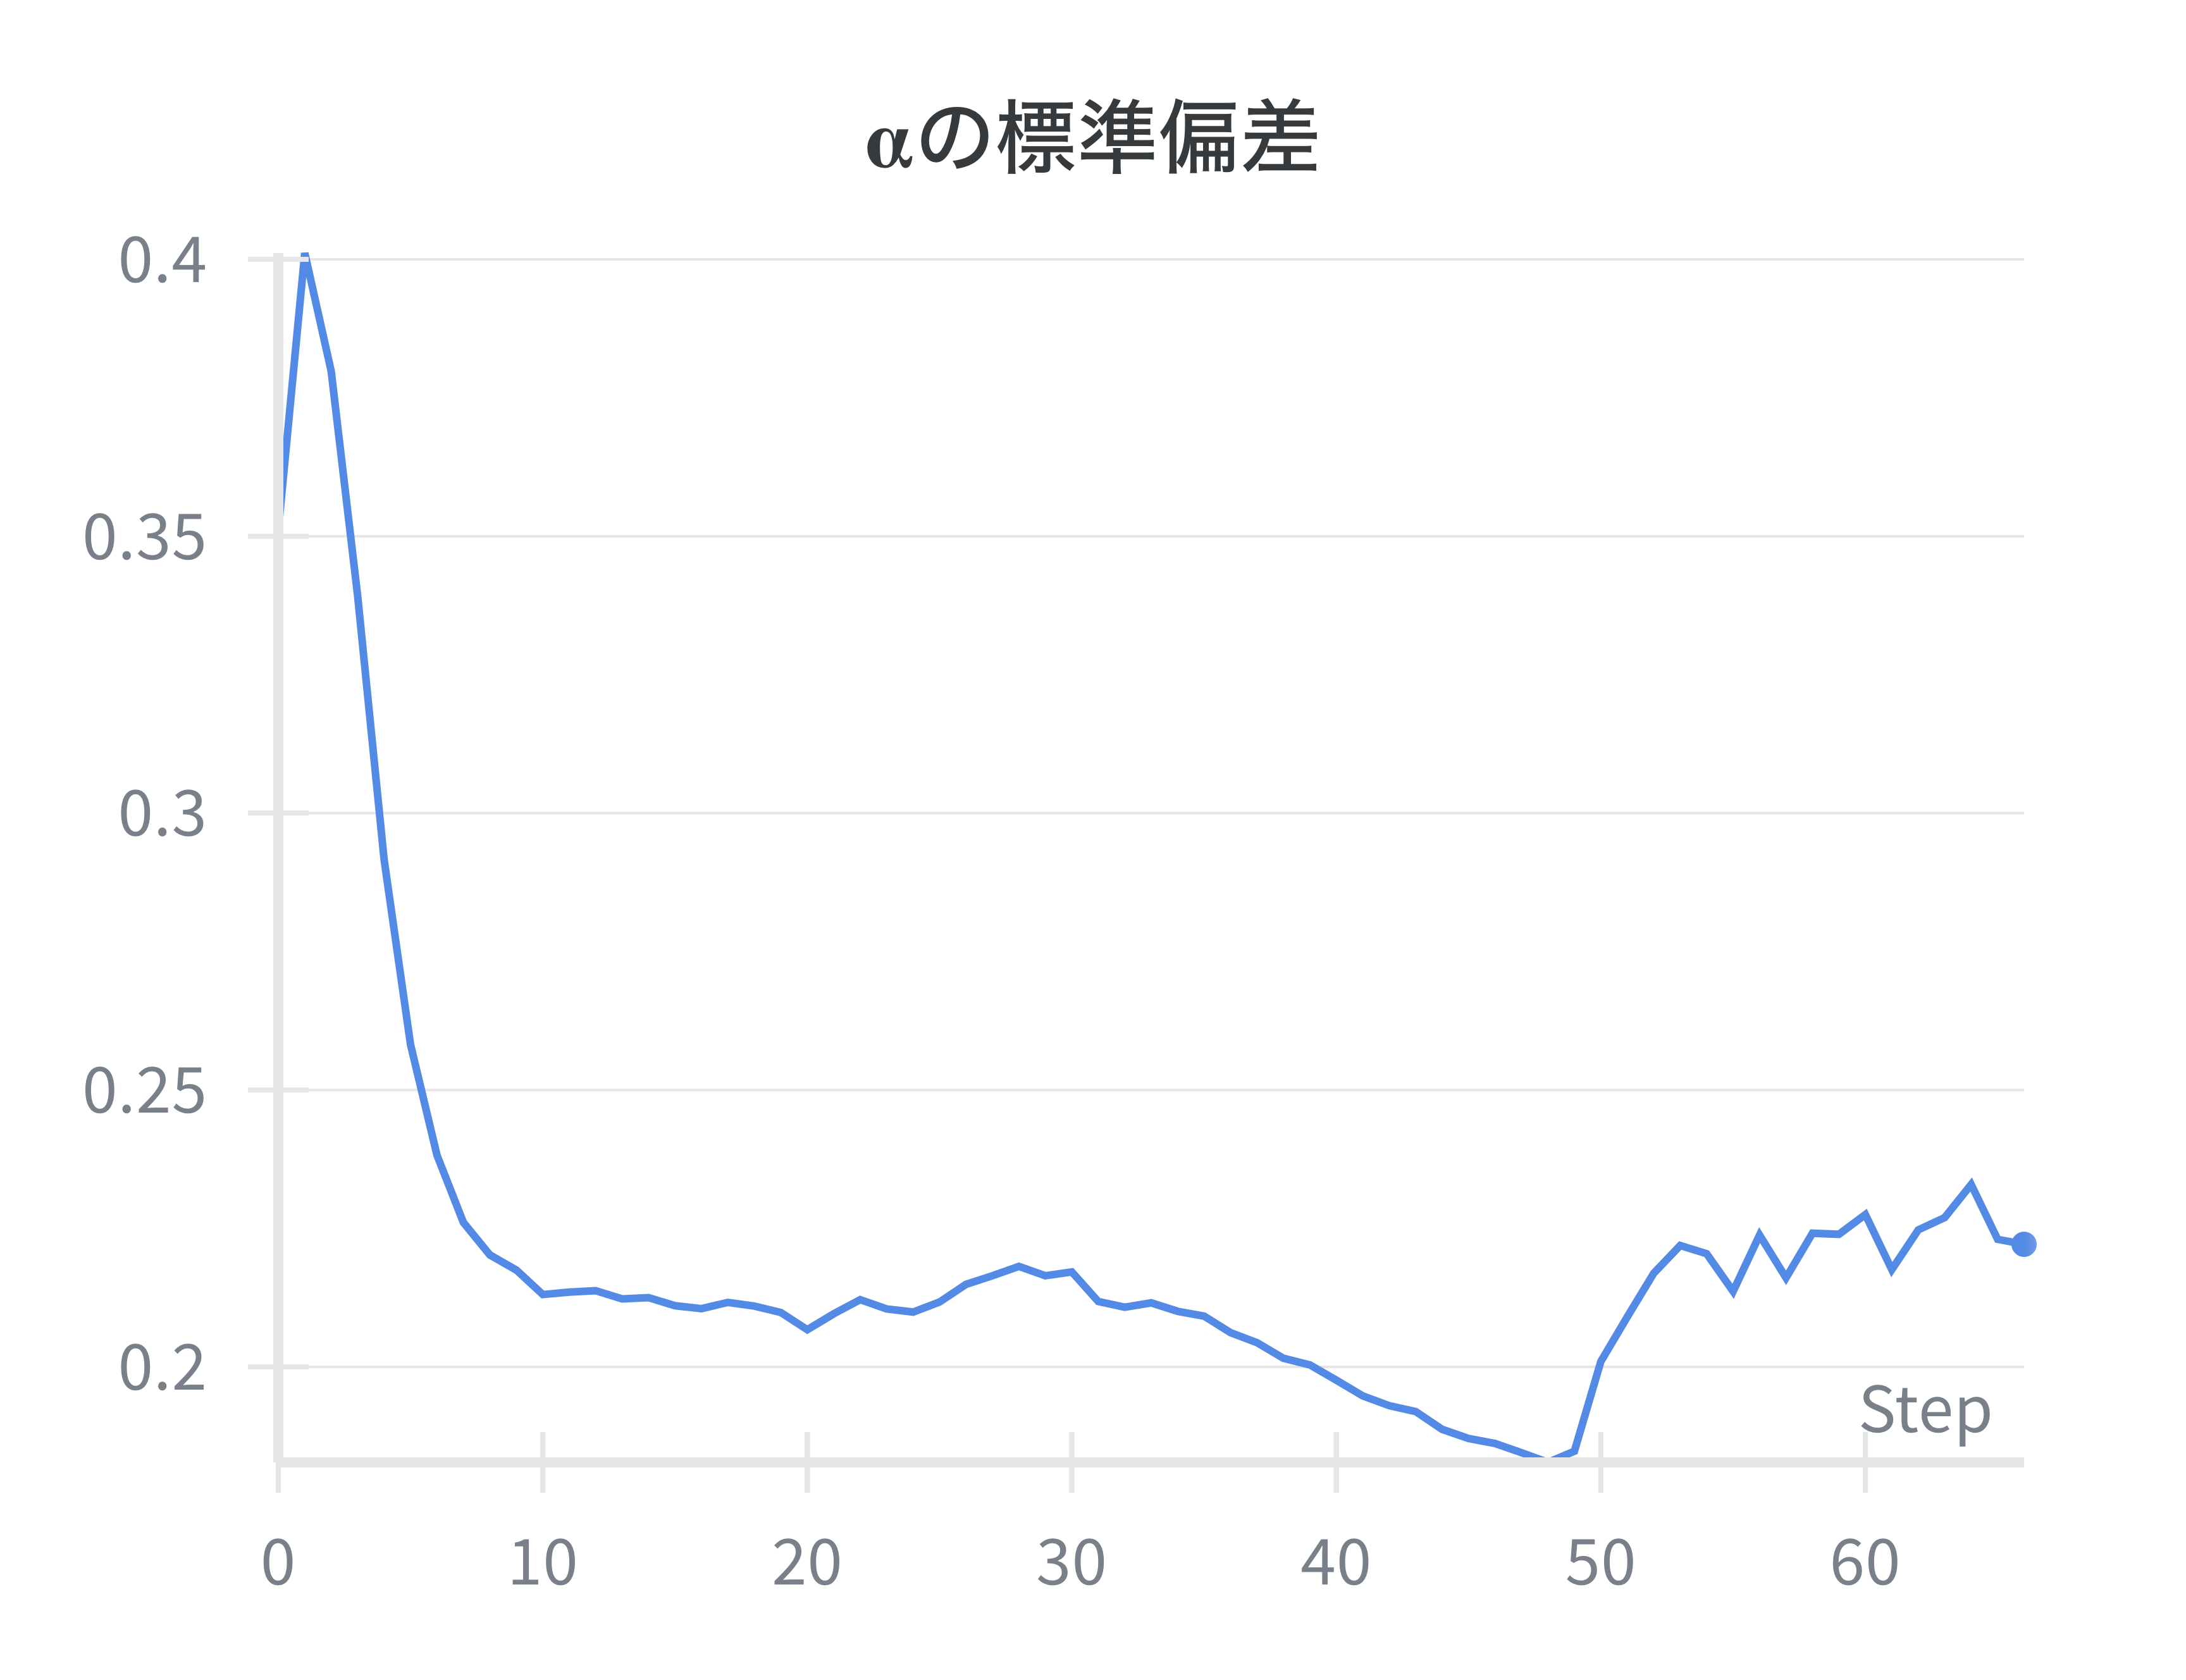
\includegraphics[width=\linewidth]{image/alpha_std.png}
    \subcaption{Std of $\boldsymbol{\alpha}$}
  \end{minipage}
  \caption{
    Gated Fusion パラメータ $\boldsymbol{\alpha}$ の学習過程における統計量の推移．
    (a) 平均値は約0.2まで低下し，多くの次元で運動特徴が抑制されていることを示す．
    (b) 最大値は常に1.0付近を維持しており，局所的には運動特徴が支配的である．
    (c) 最小値は0付近に収束している．
    (d) 標準偏差は約0.2で安定しており，次元ごとに重みが大きく異なる（選択的である）ことを示唆する．
  }
  \label{fig:alpha_stats}
\end{figure}

分析の結果，以下の特徴が明らかになった：
\begin{enumerate}
  \item \textbf{平均値の低下とノイズ抑制（図\ref{fig:alpha_stats}(a)）}：
    $\boldsymbol{\alpha}$ の平均値は学習初期の約0.5から急激に減少し，以降は約0.2付近で安定して推移している．
    これは，特徴次元全体のおよそ80\%の重みが外観特徴（RGB）に割り当てられていることを意味する．
    前節で述べた通り，本データセットにはカメラワークによる背景の動きが多く含まれるため，
    モデルは学習を通じて信頼性の低い運動情報を全体的に抑制し，
    ノイズの影響を最小限に留める戦略を獲得したと解釈できる．

  \item \textbf{決定的特徴の選択（図\ref{fig:alpha_stats}(b)）}：
    一方で，$\boldsymbol{\alpha}$ の最大値は学習全体を通じて1.0に近い値を維持し続けた．
    平均値が低いにもかかわらず最大値が高いという事実は，
    特定の少数の特徴次元においては，運動特徴（オプティカルフロー）が行動識別のための最も重要な手がかりとして
    ピンポイントで採用されていることを強く示唆している．

  \item \textbf{特徴選択のスパース性（図\ref{fig:alpha_stats}(d)）}：
    $\boldsymbol{\alpha}$ の標準偏差は初期に減少した後，約0.2前後の値を維持している．
    平均値が0.2と低い状態で，標準偏差が0.2あるということは，
    パラメータの分布が0付近に偏りつつも，一部の高い値を持つ次元が存在するという「スパース（疎）な分布」であることを意味する．
    これは，Gated Fusion が全次元を均等に扱うのではなく，
    「不要な次元はカットし，必要な次元だけを通す」という
    明確な特徴選択を行っていることの統計的な証左である．
    
  \item \textbf{考察}：
    以上の挙動は，提案手法が外観情報をベースとしつつ，
    行動の本質に関わる重要な動き情報のみを選択的に取り入れる
    「適応的統合」を実現していることを示している．
    この機構により，背景ノイズに頑健でありながら，
    必要な運動情報を見落とさないロバストな特徴抽出が可能になったと結論付けられる．
\end{enumerate}
